
The dataset used has a large affect on the total delayed neutron yield and average half-life values.
Figure \ref{fig:hybrid-pure-compare} shows how the previously discussed datasets compare to each other.
These results show that the ENDF/B-VII.1 and ENDF/B-VIII.0 datasets have delayed neutron yields $\nu_d(I)$ and average half-lives $\bar{\tau}(I)$ within uncertainty bounds of each other.
However, the ENDF results are not consistent with the results from JEFF-3.1.1, JENDL-5, and the IAEA dataset using JENDL-5 cumulative fission yields.

\begin{figure}[!ht]
\centering
\subfloat[The total delayed neutron yield.]{
  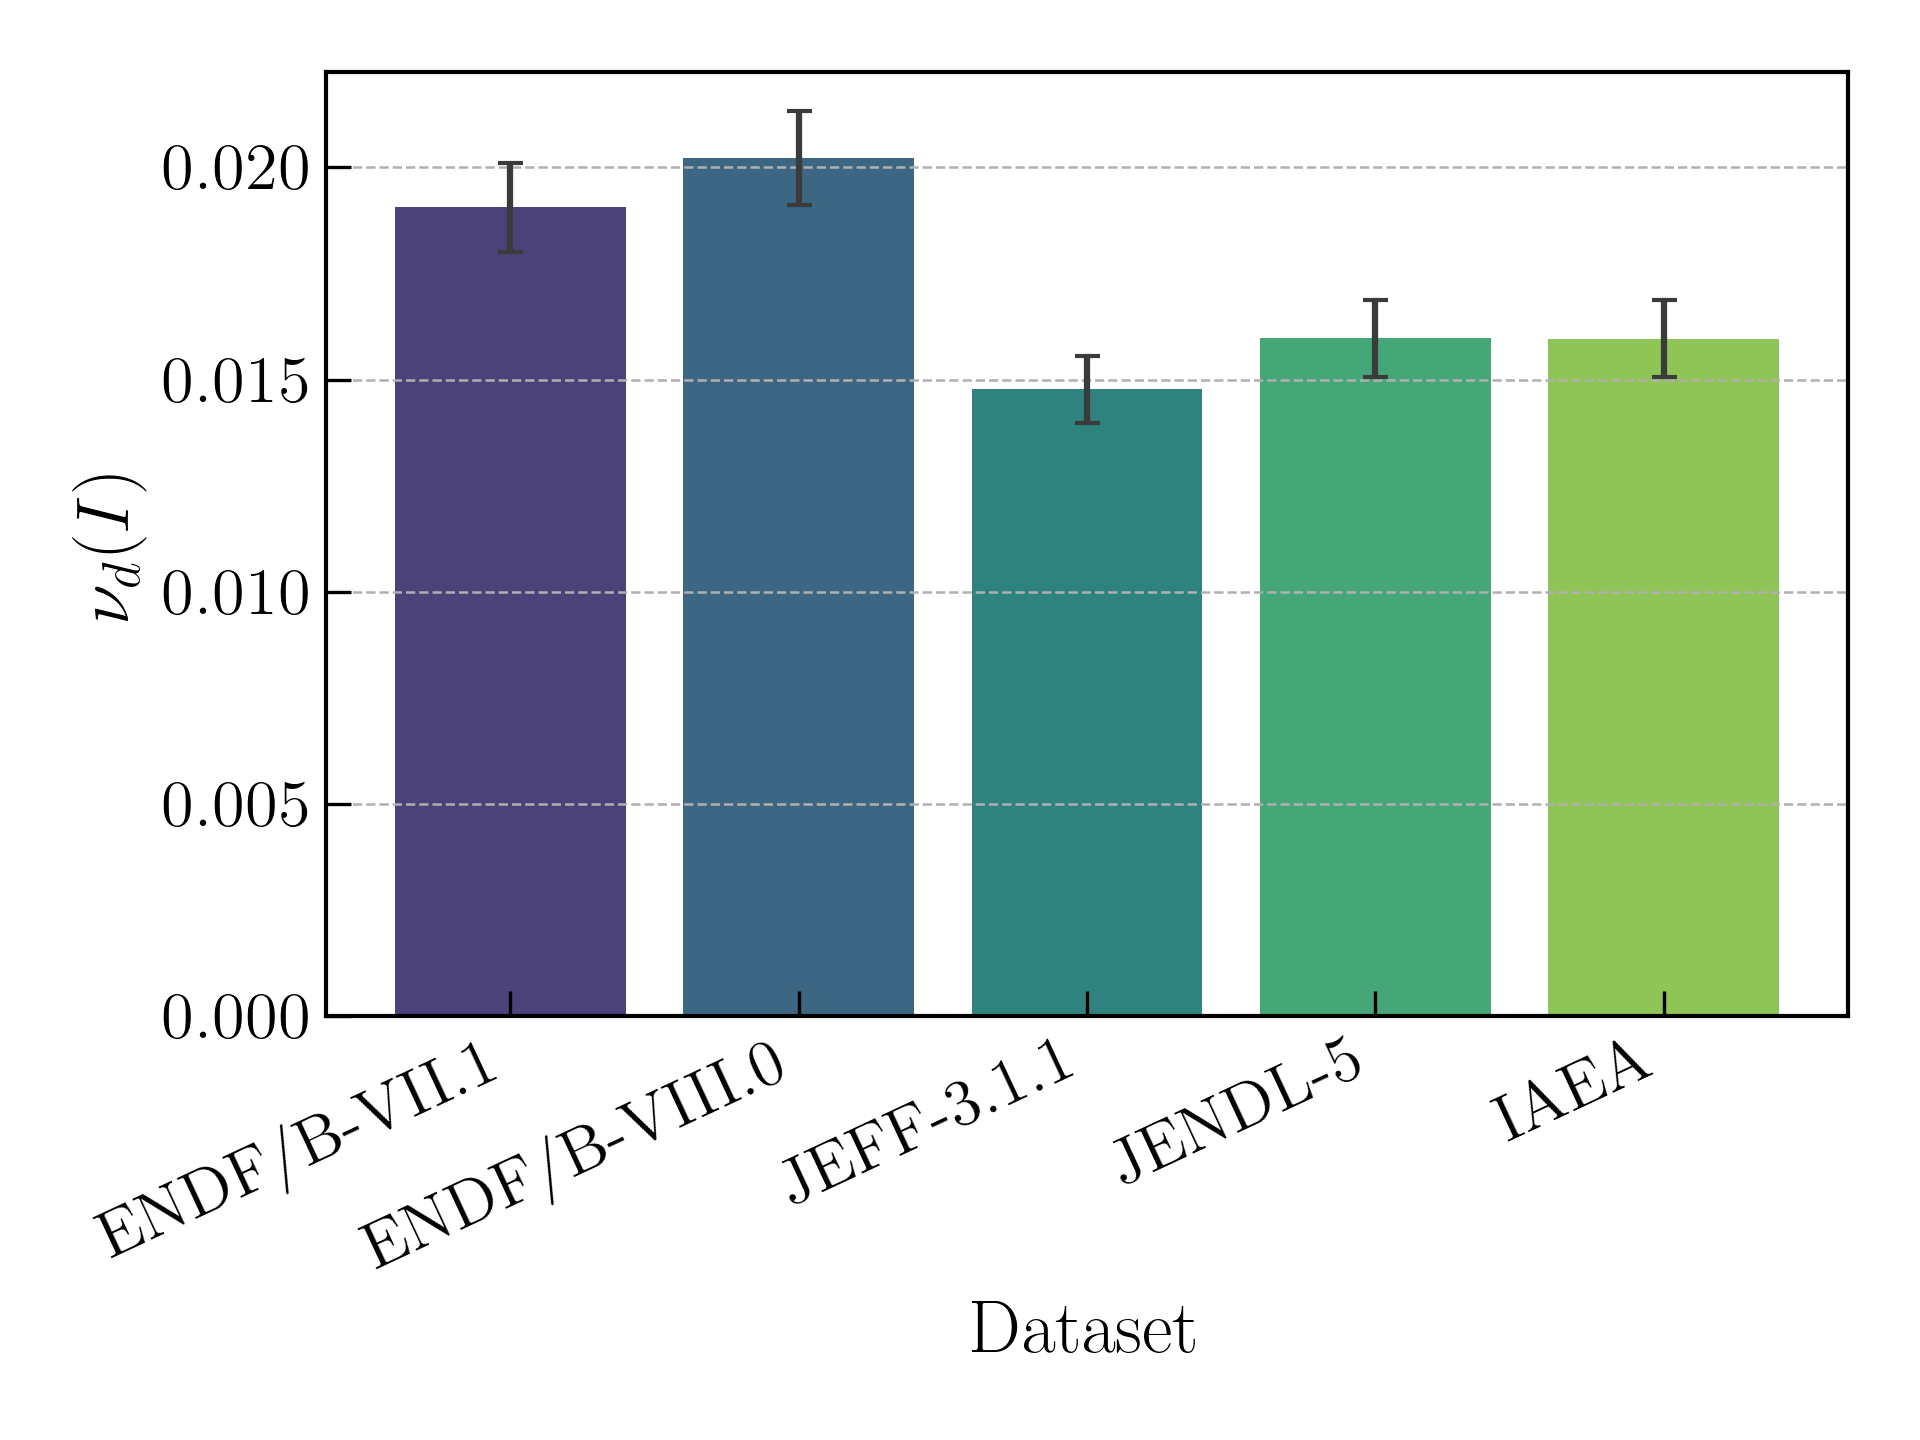
\includegraphics[width=0.45\linewidth]{images/hybrid/pure_yield_bar.png}
}
\hspace{0.05\linewidth}
\subfloat[The average half-life.]{
  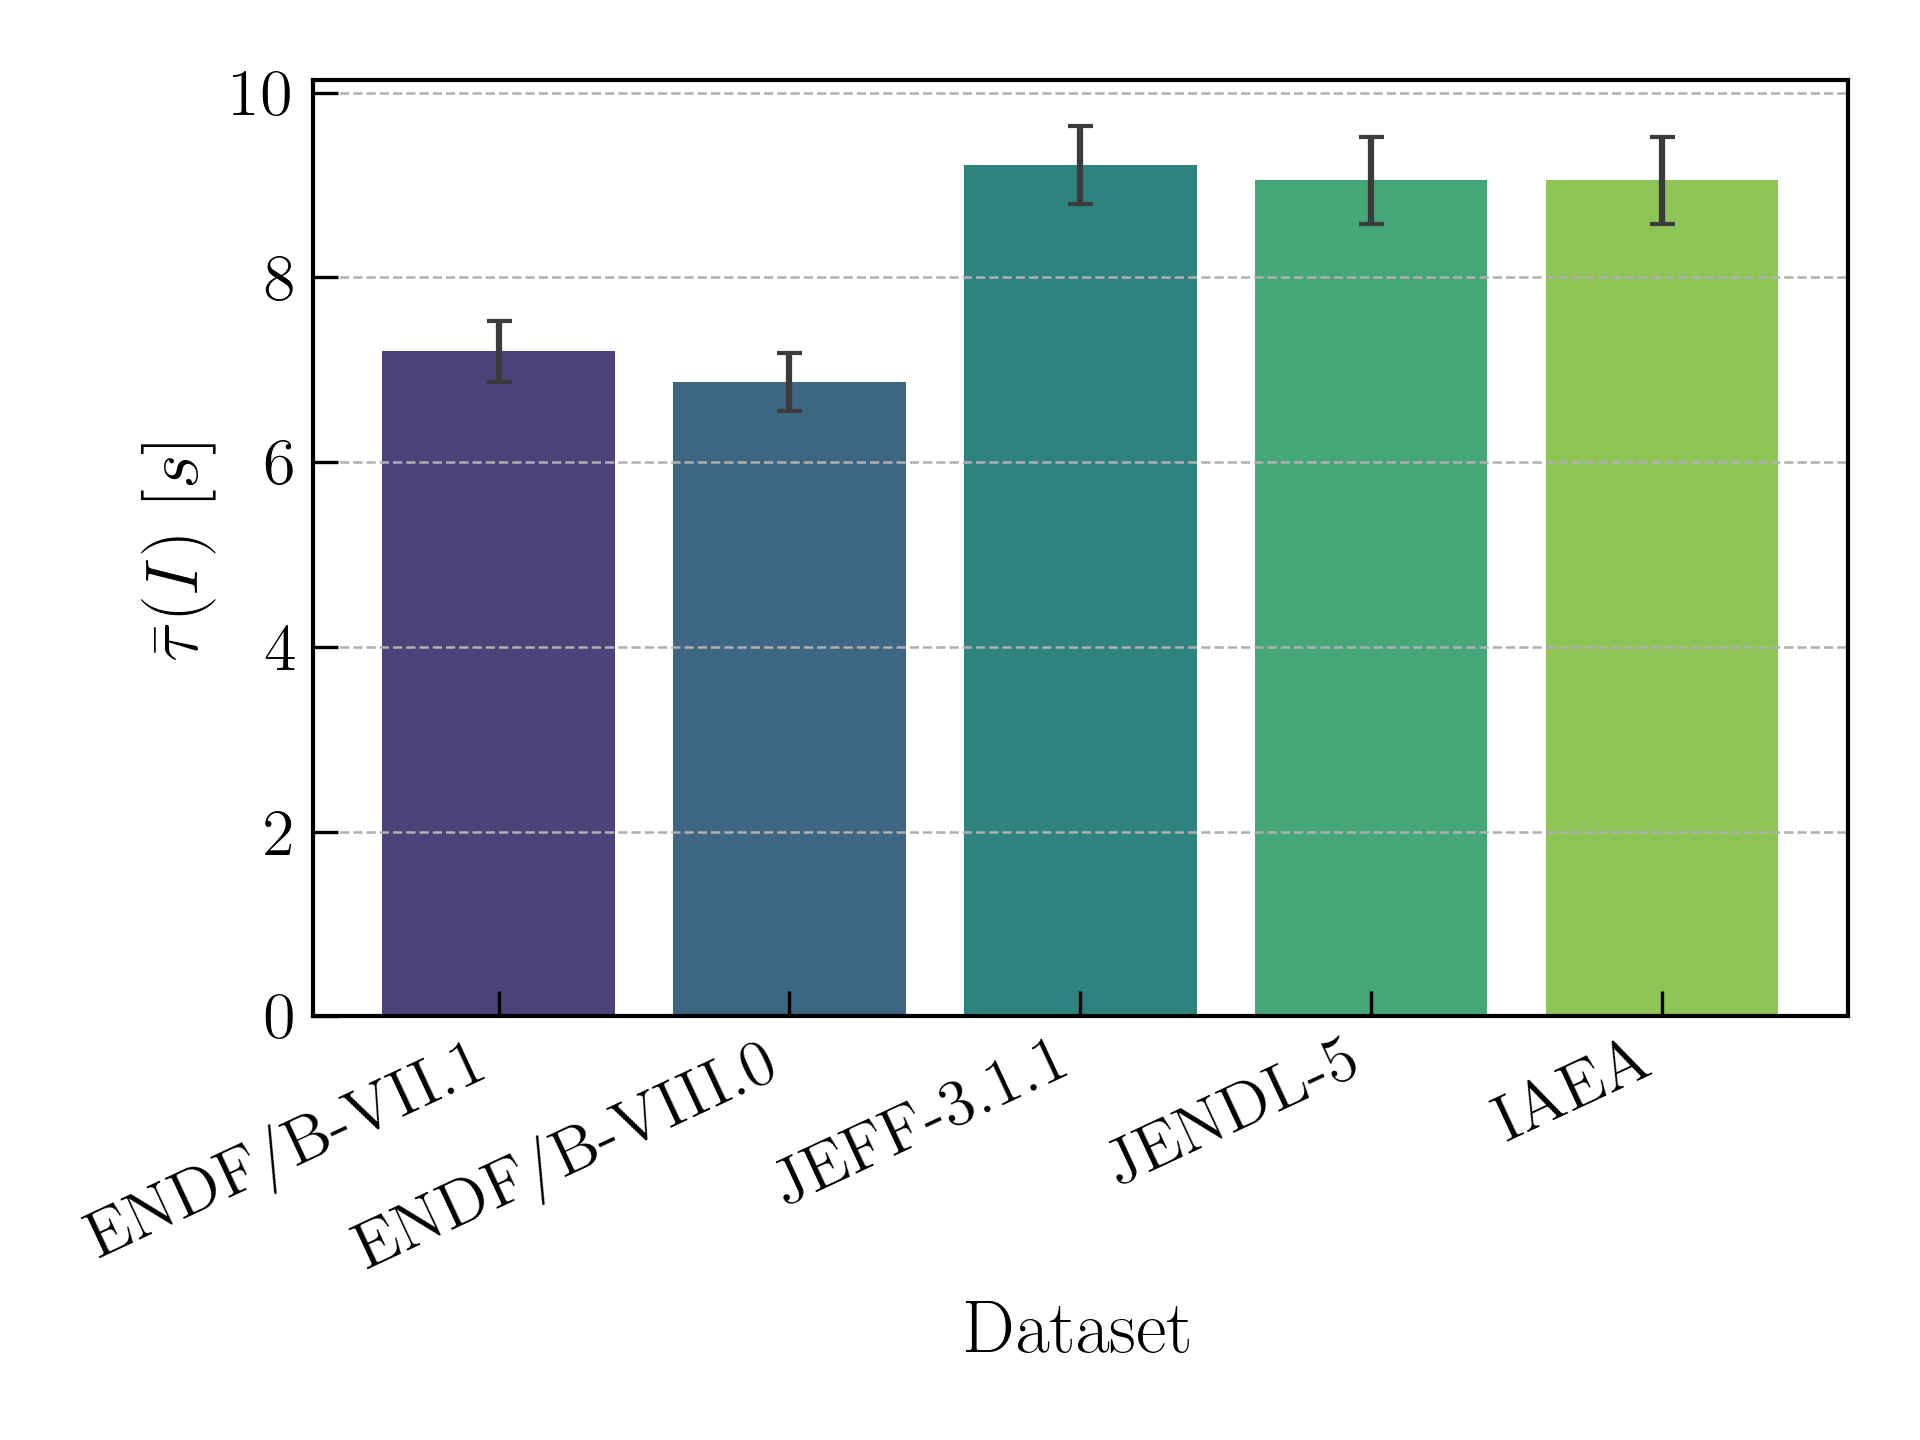
\includegraphics[width=0.45\linewidth]{images/hybrid/pure_hl_bar.png}
}
\caption{Bar charts comparing the total delayed neutron yield $\nu_d(I)$ and average half-lives $\bar{\tau} (I)$ from the previously discussed datasets.}
\label{fig:hybrid-pure-compare}
\end{figure}

Figure \ref{fig:hybrid-iaea-compare} shows how the cumulative fission yields from the different datasets affect the results when the IAEA beta-delayed neutron emission database half-lives and emission probabilities are used.
The results reflect those shown in Figure \ref{fig:hybrid-pure-compare}, where the JENDL-5 and JEFF-3.1.1 results are within uncertainty bounds while the ENDF results are within uncertainty bounds, but the two sets are not within uncertainty bounds of each other.

\begin{figure}[!ht]
\centering
\subfloat[The total delayed neutron yield.]{
  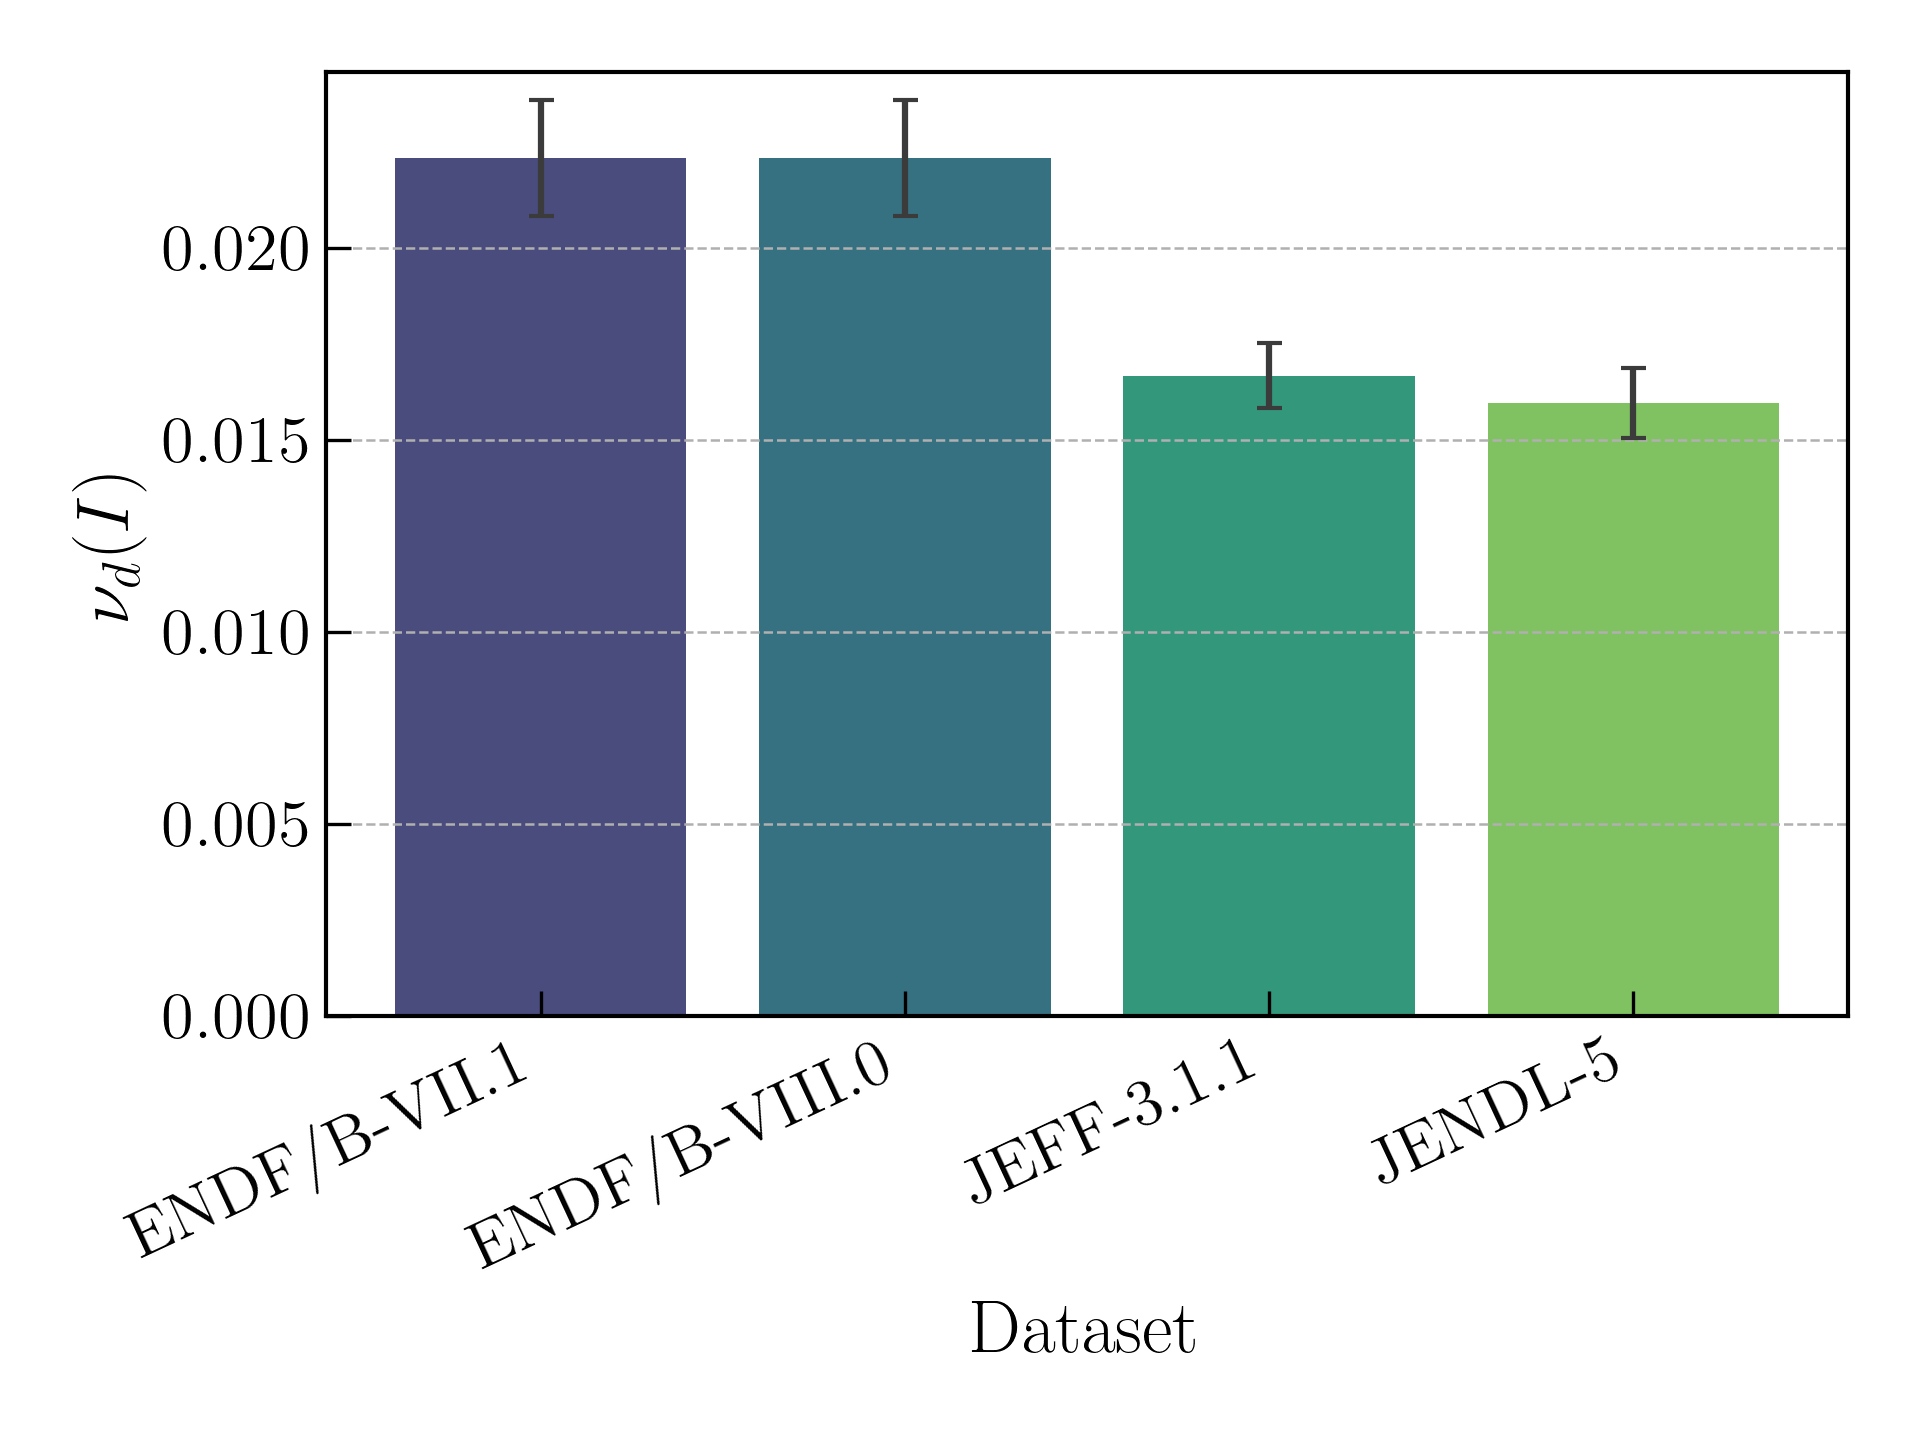
\includegraphics[width=0.45\linewidth]{images/hybrid/iaea_yield_bar.png}
}
\hspace{0.05\linewidth}
\subfloat[The average half-life.]{
  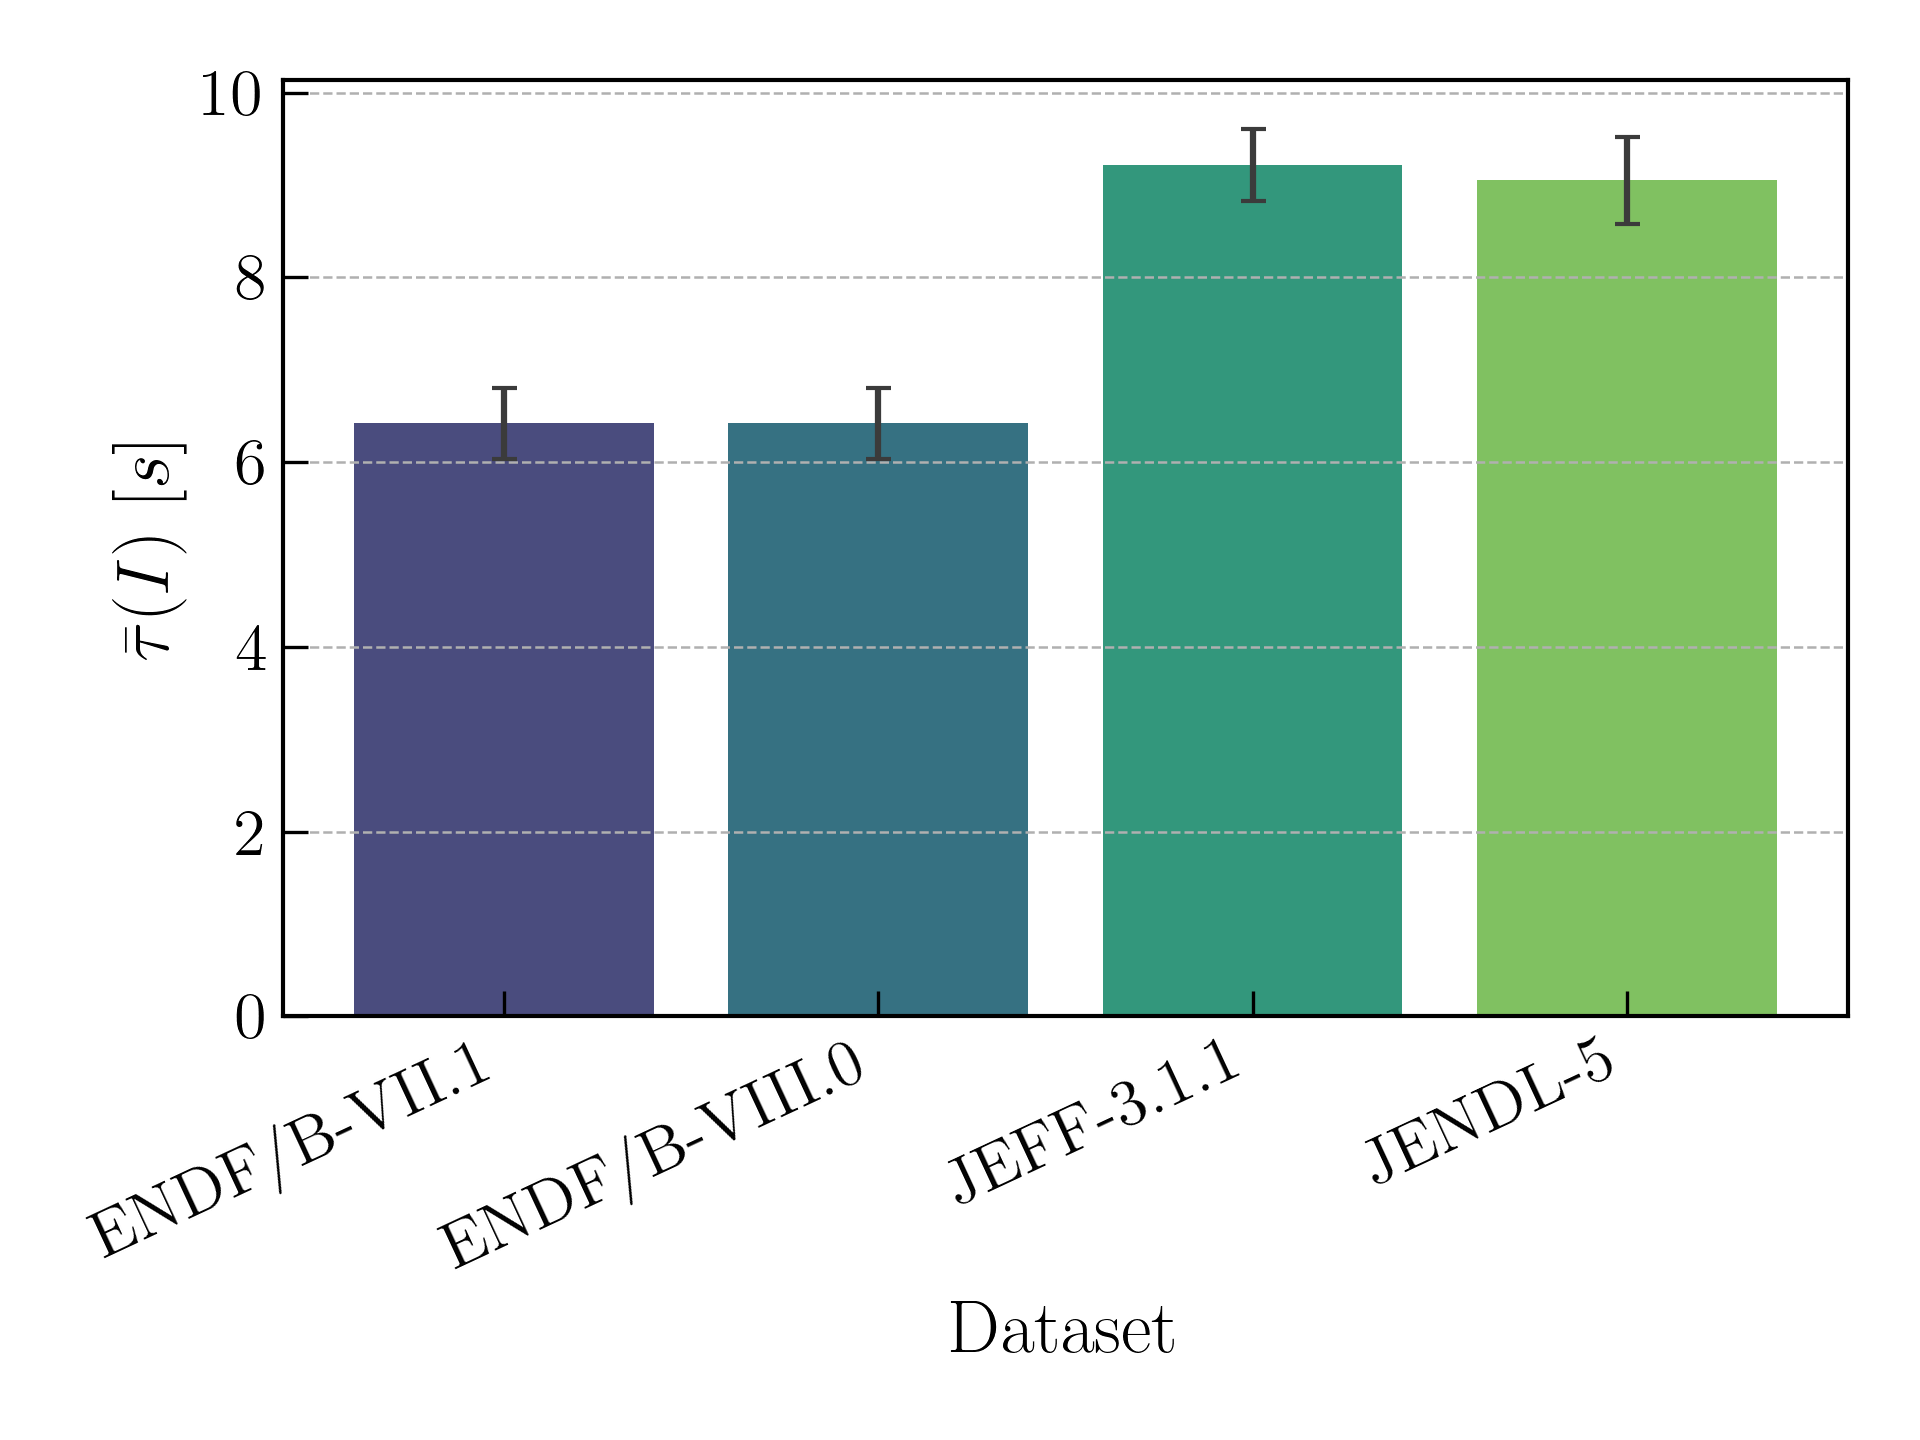
\includegraphics[width=0.45\linewidth]{images/hybrid/iaea_hl_bar.png}
}
\caption{Bar charts comparing the total delayed neutron yield $\nu_d(I)$ and average half-lives $\bar{\tau} (I)$ using the IAEA beta-delayed neutron emission database half-lives and emission probabilities for differing cumulative fission yield datasets.}
\label{fig:hybrid-iaea-compare}
\end{figure}


However, it is also possible to combine datasets, mixing the cumulative fission yields, emission probabilities, and half-lives.
Figure \ref{fig:hybrid-nu-heatmap} shows heatmaps of the total delayed neutron yield $\nu_d (I)$ plotted against different cumulative fission yield and emission probability datasets.
Although it is expected that the half-life dataset should not have an effect, only the nuclides present in all three datasets is included.
This means that using the JEFF-3.1.1 half-lives results in a decrease to the total delayed neutron yield due to missing \gls{DNP} present in the ENDF datasets.
Interestingly, this has a larger effect on the ENDF cumulative fission yield calculated delayed neutron yields compared to those from JEFF-3.1.1 and JENDL-5.
This is because the ENDF data has large \glspl{PCC} for certain \glspl{DNP}, such as $^{88}$As, that are not included in JEFF-3.1.1.
This indicates the cumulative fission yields for these \glspl{DNP} may be over-reported in ENDF data compared to JENDL-5 and JEFF-3.1.1.

\begin{figure}[!ht]
\centering
\subfloat[The total delayed neutron yield using ENDF/B-VII.1 half-lives.]{
  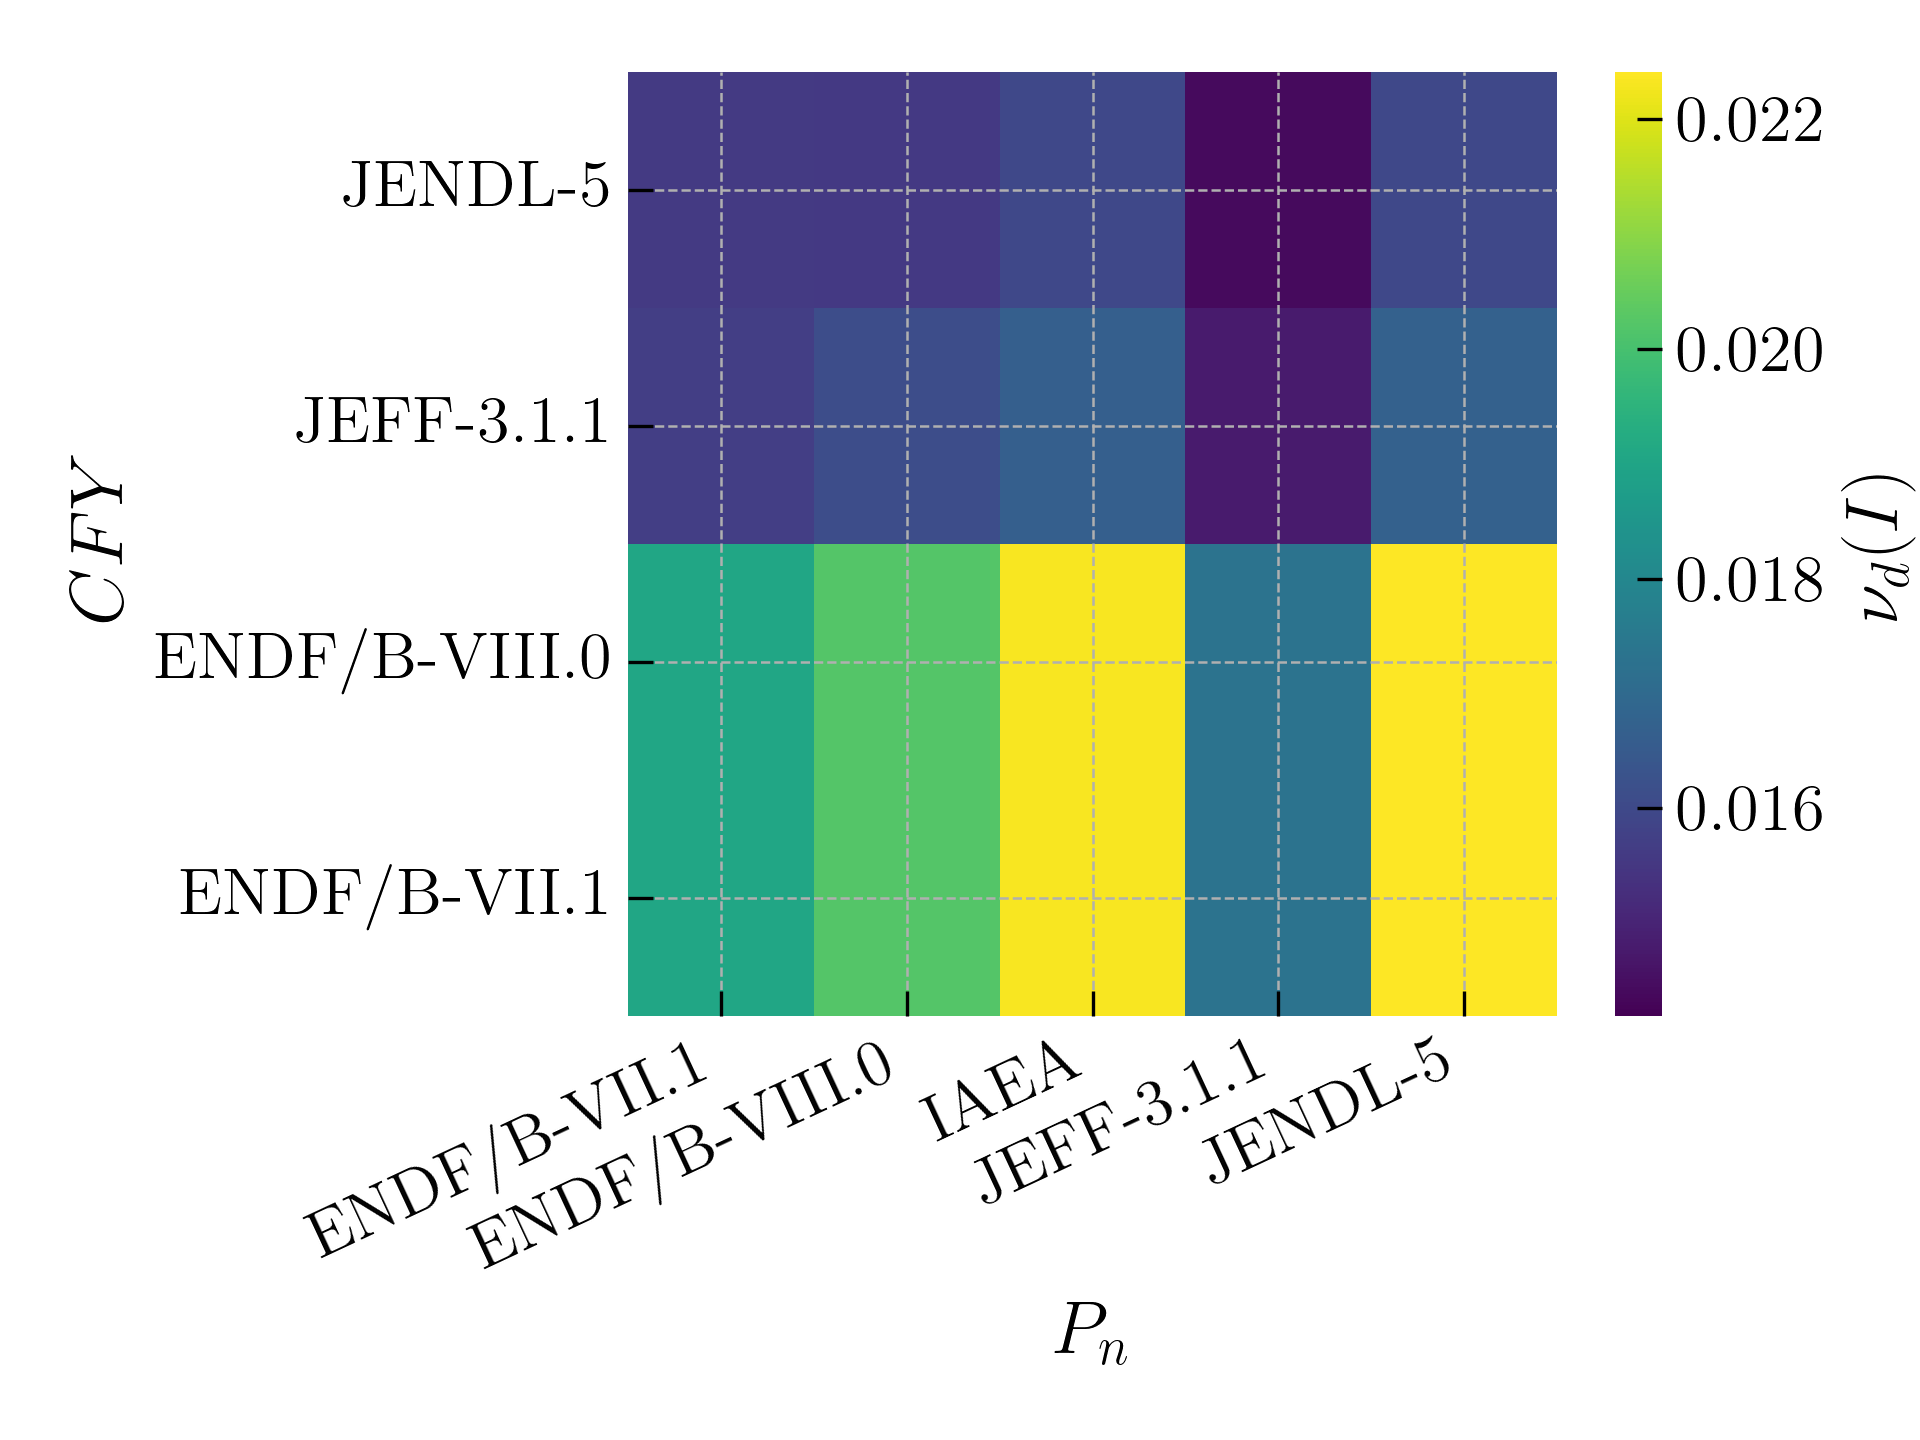
\includegraphics[width=0.45\linewidth]{images/hybrid/yield_surf_tau_ENDFB-VII.1.png}
}
\hspace{0.05\linewidth}
\subfloat[The total delayed neutron yield using JEFF-3.1.1 half-lives.]{
  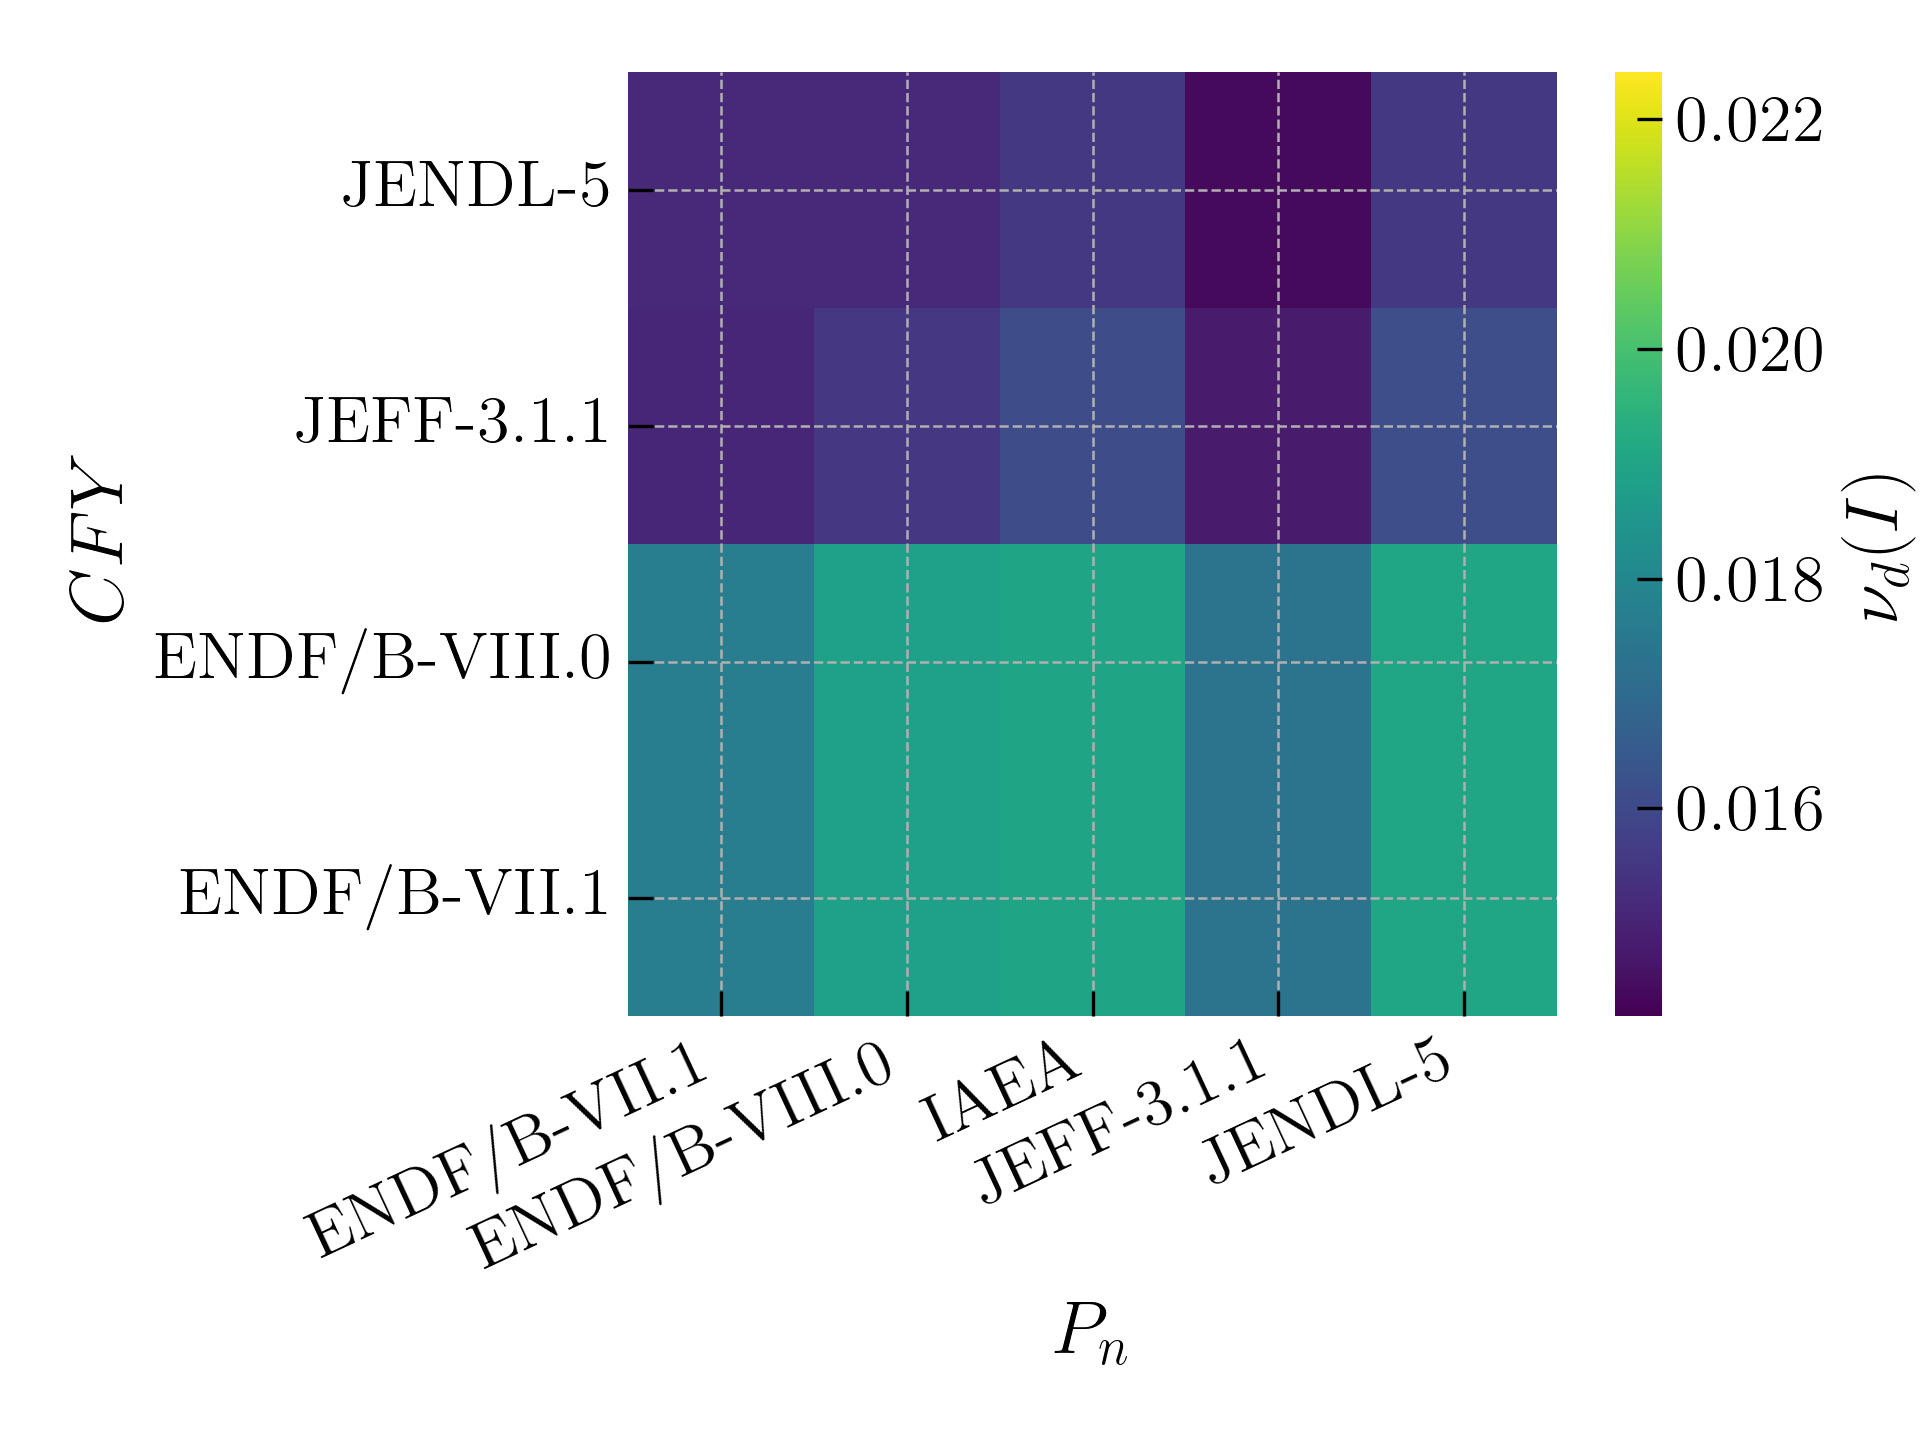
\includegraphics[width=0.45\linewidth]{images/hybrid/yield_surf_tau_JEFF-3.1.1.png}
}
\caption{Heatmaps of the total delayed neutron yield $\nu_d (I)$ calculated using various datasets for the cumulative fission yield, emission probability, and half-life.}
\label{fig:hybrid-nu-heatmap}
\end{figure}

It appears in Figure \ref{fig:hybrid-nu-heatmap} that the cumulative fission yield differences are what drive the differences in the total delayed neutron yields, with smaller differences from the emission probabilities.
This is useful to note, as based on the uncertainty-weighted \glspl{PCC} calculated in Sections \ref{sec:b71} and \ref{sec:b80}, the emission probability data is the data in most need of updating.
This is because the ENDF data has smaller relative uncertainties for the cumulative fission yields even though they do not agree well with the JEFF-3.1.1 and JENDL-5 cumulative fission yields.

Table \ref{tab:total-delnu-compare-net} shows how total delayed neutron yields from the literature calculated using summation approaches or from experimental data compare with the results from this work.
Among the values shown in Table \ref{tab:total-delnu-compare-net}, the outliers are the ENDF/B-VII.1 and ENDF/B-VIII.0 $\nu_d$ values.

\begin{table}[!h]
    \centering
    \caption{Total delayed neutron yields $\nu_d$ of 100 fissions from thermal fission of $^{235}$U (based on \cite{huynh2014calculation}).}
    \begin{threeparttable}
    \begin{tabular}{ll}
        \hline
       Data & $\nu_d$ $[-]$ \\
       \hline
        JEF-2.2 \cite{bank2000jef, huynh2014calculation} & $1.708 \pm 0.12$\\
        JEF-3.1.1 \cite{santamarina2009jeff, huynh2014calculation} & $1.477 \pm 0.08$\\
        ENDF/B-VII.1 \cite{chadwick2011endf, huynh2014calculation} & $1.905 \pm 0.10$\\
        Keepin et al. \cite{keepin1957delayed} & $1.580 \pm 0.07$ \\
        Charlton et al. \cite{charlton1996delayed} & $1.577 \pm 0.03$\\
        Saleh et al. \cite{saleh1997measurements} & $1.645 \pm 0.11$ \\
        Synetos and Williams \cite{synetos1983delayed} & $1.510 \pm 0.06$ \\
        Tuttle \cite{tuttle1975delayed} & $1.700 \pm  0.05$\\
        Waldo et al.\cite{waldo1981delayed} & $1.670 \pm 0.07$ \\
        \hline
        IAEA/JENDL-5 \cite{DIMITRIOU2021144, iwamoto2023japanese} & $1.596 \pm 0.09$\\
        ENDF/B-VII.1 \cite{chadwick2011endf} & $1.906 \pm 0.11$\\
        ENDF/B-VIII.0 \cite{Brown20181} & $2.023 \pm 0.11$\\
        JEFF-3.1.1 \cite{santamarina2009jeff} & $1.477 \pm 0.08$\\
        JENDL-5 \cite{iwamoto2023japanese} & $1.597 \pm 0.09$ \\
        \hline
    \end{tabular}
    \label{tab:total-delnu-compare-net}
    \end{threeparttable}
\end{table}

The results thus far have indicated potential discrepancies in the ENDF cumulative fission yields for \glspl{DNP}.
To investigate this, cumulative fission yield differences between JENDL-5 and ENDF/B-VIII.0 are compared for the \glspl{DNP} with the largest delayed neutron yield $\nu_d(I)$ contribution differences.
This analysis showed there are two \glspl{DNP} alone that account for 67\% of the delayed neutron yield difference: $^{86}$As and $^{137}$Sb.
The $^{86}$As yield difference primarily comes from the cumulative fission yield difference, which is $540 \pm 90$ $pcm$ larger in ENDF/B-VIII.0 than JENDL-5, and leads to a delayed neutron yield difference of $191 \pm 32$ $pcm$.

The $^{137}$Sb yield difference has several contributing components: the emission probability in JENDL-5 is $0.49 \pm 0.08$, while the emission probability in ENDF/B-VIII.0 is $1.0 \pm 0.0$\footnote{No uncertainty is given, so an uncertainty of $1 \times 10^{-12}$ is used.}; the half-life in JENDL-5 is $0.94 \pm 0.01$ seconds, while the half-life in ENDF/B-VIII.0 is $0.45 \pm 0.05$ seconds; and finally the cumulative fission yield in JENDL-5 is $(2.4 \pm 0.9) \times 10^{-5}$, while the cumulative fission yield in ENDF/B-VIII.0 is $(7 \pm 5)\times 10^{-4}$.
There are other \glspl{DNP} that contribute to the total delayed neutron yield discrepancy between ENDF and the other data sets, such as the cumulative fission yield of $^{85}$As, the cumulative fission yield of $^{90}$Br, all of the data for $^{86}$Ge, the cumulative fission yield of $^{94}$Rb, the cumulative fission yield of $^{137}$I, the cumulative fission yield and half-life of $^{98m}$Y, and others.
Of the \glspl{DNP} listed, only $^{94}$Rb and $^{137}$I have larger yields in JENDL-5 than in ENDF/B-VIII.0; most of the differences in the nuclear data for \glspl{DNP} lead to ENDF datasets having a larger delayed neutron yield. 

